% ============================================== %
% PROPOSED METHODS %
% ============================================== %

\vspace{-7pt}
\subsection{Predictive Interval for Adaptive Bounds}
\label{subsec:adaptive-pruning}
%Premble


%% I_u and its drawbacks
In general, both the pruning schemes provided by DiVE-Greedy and DiVE-dSwap rely on the fundamental idea of evaluating the upper bound of the benefit provided by a view $V_i$ towards the objective $F$. 
%
If that maximum benefit is still not enough to consider $V_i$ to join $S$, then $V_i$ is pruned and its query processing cost is saved. 
%
Moreover, to evaluate that upper bound, both schemes compute the actual diversity offered by $V_i$ and instead of computing its actual importance, it is substituted with the maximum attainable importance score $I_u$. 
%
Naturally, overestimating  $I(V_i)$ leads to overestimating its benefit and consequently limited pruning power is achieved. 
%
Meanwhile, for most datasets, $I_u$ is in fact an overestimation of $I(V_i)$. 
%
Hence, our goal in this section to provide a tighter bound on $I(V_i)$, which allows for maximum pruning while maintaining the quality of the solution. 
 

Recall that $I_u$ is achieved when for each group $a_i$, the corresponding value $\frac{g_i}{G}$ in $P[V_{i}(D_R)]$ or $P[V_{i}(D_Q)]$ is zero. 
%
Hence, $I_u$ is a theoretical bound for the maximum importance achieved by any view in any dataset.
%
For most real datasets, however, that condition is rarely satisfied and the actual upper bound $I_{au}$ is typically much smaller than $I_u$. 
%
Meanwhile, a hypothetical pruning scheme that utilizes that actual upper bound $I_{au}$ is expected to deliver more pruning power than the schemes using the theoretical upper bound $I_u$, especially when $I_{au}  \ll I_u$.
%
In practice, however, that hypothetical scheme is not achievable since obtaining the value $I_{au}$ requires executing all the possible views, which is clearly in conflict with the goal of pruning.

Accordingly, rather than using overestimated $I_u$ or obtaining the actual $I_{au}$, our goal is to estimate $I_{au}$ with high accuracy and minimum number of query executions. 
%
In particular, given the set of possible views $\mathbb{V}$, the goal is to estimate the maximum importance $\bar{I}_{au}$ given by some view in $\mathbb{V}$. 
%
However, estimating the maximum value of a population is known to be a challenging problem, as opposed to estimating other statistics such as average or sum \cite{Hu:2009:EAT:1516360.1516487}.
%
That challenge is further emphasized when the values exhibited by the population are skewed and do not follow a typical normal distribution, which is typically the case for the importance value of views.
 %
 
Thus, instead of estimating $I_{au}$, we rely on {\em non-parametric predictive interval} models to determine its value with certain level of confidence without any assumption on the population \cite{Hu:2009:EAT:1516360.1516487}. 
%
To apply that model, some sample views are executed and the maximum importance observed in that sample is recorded as $\bar{I}_{au}$. 
%
To determine the number of samples, a {\em Predictive Interval (PI)} is to be defined, such that: 	
$PI= \dfrac{\left(m-1\right) }{\left(m + 1\right)}$, where $m$ is the number of samples. 
%

For instance, setting $m = 19$, results in PI = 90\%. 
%
That is, 90\% of the time, the importance value of an unseen view $V_i$ will be less than the maximum importance seen so far. 
%
Clearly, the higher the PI value, the higher the accuracy of $\bar{I}_{au}$, but also requires executing more views.  
%
In this work, we find that a value of $PI=97\%$ is able to strike a fine balance between minimizing the number of executed queries and maximizing the objective $F$, as shown next.


\eat{
Two pruning techniques \textit{DiVE-Greedy-Static} and \textit{DiVE-dSwap-Static} have been presented. Those two static pruning techniques utilized maximum bound $I_u$ to determine whether the query view need to be executed or not. Only view that can improve the $F(S)$ of the current set while using $I_u$ will be executed otherwise those are pruned. However, one drawback using static bound $I_u$ in pruning technique is that if the bound is far away from the maximum score of importance score in the dataset, the pruning cannot work optimal. To overcome this issue, instead of using static bound $I_u$, we proposed adaptive pruning scheme that automatically adapts the bound to the real maximum importance score in the dataset. 

The adaptive pruning technique is utilizing the maximum bound $I_u$ as in static pruning as a first initial bound, however, this bound is changed to the real value of maximum importance score after some query views are executed. The problem occurs when the executed views have a small importance score and it is far below from the most views in the dataset. Thus, it brings the pruning out of control because while the bound is very low and there are many views in dataset have higher importance score compared to the bound, it may result wrong prune. Hence, DiVE needs the strategy to ensure that the bound score is close as possible to the maximum importance score in the dataset while it is changed. One of the approach that can be used is by selecting sample views to be executed then get the maximum importance score of the view from those sample. This brings us to the question of how many samples are needed in order to hit a view that has a maximum score from the dataset.

There are several literatures have been mentioned related to the confidence interval and the number of samples in the normal distribution [cite]. However, the importance score of candidate views in $X$ is not in normal distribution. The highest importance score is the upper bound of maximum importance $I_u$ whereas the lowest is 0, and it is long tail distribution. Hence, we adopt the sampling method from this [cite] as our data is not in normal distribution, it is called as prediction interval ($ PI $) which is similar to a confidence interval in normal distribution. The relation between $ PI $ and the number of samples defined as in equation \ref{prediction-interval}.

\begin{equation}
	PI= \dfrac{\left(N-1\right) }{\left(N + 1\right)}, where\, N = Number\, of\, samples
	\label{prediction-interval}
\end{equation}

In general, analyst may use $ PI $ start from 80 to 99. While $ PI $ = 80\% states that there are 9 sample views need to be executed, 85 \%, 90\%, 95\%, 97\%, and 99\% means 12, 20, 40, 60, and 200 samples need to be executed respectively. 

\textit{Adaptive pruning flows}. We employ adaptive pruning technique to both schemes, \textit{DiVE-Greedy} and \textit{DiVE-dSwap}. In case of Greedy technique, the upper bound $I_u$ is used at the first time, thus the value $I_u$ is changed to maximum importance score from the samples of views which are executed. In order to change the bound value, the number of samples that need to be executed depends on the $ PI $ value which defined by the analyst. Futhermore, the bound is changed while in the next view execution that there is a view which has importance score higher than the used current bound.

For adaptive pruning technique in \textit{DiVE-dSwap}, the details is described as follows:

\begin{itemize}
	\item Firstly, as in \textit{ DiVE-dSwap-Static} that all query view in the initial set are executed in order to get the objective function $F(S)$ of the current set $S$ and all candidate views in $X$ is sorted based on $ setDist\left(V_i, S\right)  $.
	\item $ maxU' $ of each view is computed by utilizing the maximum bound of importance score $I_u$, where $ maxU'\left(V_i\right)= \left(1-\lambda\right) \times I_u\left(V_i\right) + \lambda \times setDist\left(V_i, S\right) $. 
	\item All views in $X$ is exchanged to the current set one by one and a view that can improve $F(S)$ will be executed in order to get the actual value of importance. 
	\item The bound is changed while the number of views which are executed reaches the number of sample based on the PI which determined by analyst. For instance, analyst may use PI = 97\%, hence, bound is changed while the sum of number of candidate views and th number of views in the initial set equal to 60 views. While it reaches to 60 views, the bound is replaced by the maximum importance score of executed views.  
	\item If in the next query view execution, there is a view which has higher importance score than the bound. Thus, the bound is changed to that score. 
\end{itemize}

%To check the performance of our proposed pruning techniques

In this work, adaptive pruning in Greedy is called \textit{DiVE-Greedy-Adaptive} wheras in Swap is called \textit{DiVE-dSwap-Adaptive}.
}
%
%
%$maxU'$ of each candidate view is computed first using $current bound$ before executing the query, view which cannot make an improvement to the S while using $current bound$ will never be executed and it will be pruned
%  
%In order to get better performance of pruning scheme, instead of using static $max_I = \sqrt{2} $, we proposed Adaptive Pruning scheme, that can adapt the value of $max_I$ to the real values in the dataset. In order to estimate the $max_I$ which can close to the real value in the dataset, we use sampling method. 


%For instance, in the \textit{DiVE-dSwap-Adaptive-Pruning}, $max_I$ is initialized by $ \sqrt{2} $. If the view by using $max_I$ can improve the objective function value in the current set $S$, the real Importance score of this view will be computed which is by executing the query of its view. For instance, after executing its query, the real Importance value is 0.25, by using $ \alpha= 0.8 $, the $ EWMA_t  $ will be $ (0.8 *0.25) + ((1- 0.4)*\sqrt{2}) = 0.48 $, and the current $max_I$ will be set to 0.48, and it will be updated continuously. This EWMA method able to set the value of $max_I$ as close as the real values in the dataset, it should make pruning scheme works better. 

% % Pruning Pseudocode

%\begin{algorithm}
%	%	\SetAlgoLined
%	%	\KwIn{Set of views V and result set $S$ize k }
%	%	\KwOut{Result set $ S \geq V $, |S| = k}  
%	%	$S \leftarrow $ Result set of only importance or only diversity\;
%	%	$X \leftarrow  \left[V \backslash S\right]$\;
%	%	$F_{current} \leftarrow 0 $\;
%	%	$  improve \leftarrow  True $\;
%	$ max_b  \leftarrow\sqrt{2} $\;
%	%$ X' \leftarrow [] $\;
%	\For{$i$ in set $X$}{
%		\For{$j$ in set $S$}{
%			$ d  \leftarrow setDist\left(X[i],S \backslash S[j]\right) $\;
%			$ 	newX \leftarrow [S[j], X[i], d]$\;
%			$ 	X'.append(newX)$\;
%		}
%	}
%	$ 	X' \leftarrow sorted\_by\_d(X') $\;
%	$ S' \leftarrow S $\;
%	\eIf{ $ max_b == \sqrt{2} $}{
%		\For{$i$ in set $X'$}{
%			
%			\If{ $ F\left(S'\right) < F\left(S \backslash X'[i][0] \cup X'[i][1], max_b\right) $}{
%				$ 	X''.append(X'[i][1])$\;
%			}
%		}
%		
%		$n \leftarrow pi - len(S)$\;
%		$samples \leftarrow X''[0\colon n]$\;
%		$maxI\_S \leftarrow get\_maxI(S)$\;
%		$maxI\_samples \leftarrow get\_maxI(samples)$\;
%		
%		\If{ $ maxI\_S > maxI $}{
%			$ maxI \leftarrow maxI\_S$
%		}
%		\If{ $ maxI\_samples> maxI $}{
%			$ maxI \leftarrow maxI\_samples$
%		}
%		$max\_b \leftarrow maxI$	
%		
%		\For{$i$ in set $X''$}{
%			\For{$j$ in set $S$}{
%				\If{ $ F\left(S'\right) < F\left(S \backslash S[j] \cup X''[i], max_b\right)  $}{
%					$ 	X'''.append(X''[i])$\;
%					$ I \leftarrow get\_I\_score(X''[i]) $\;
%					\If{ $ F\left(S'\right) < F\left(S \backslash S[j] \cup X''[i], I\right) $}{
%						$ S'  \leftarrow S \backslash j \cup X''[i] $  \;
%					}
%					\If{ $ I > max_b $}{
%						$ max_b \leftarrow I $
%					}
%				}
%			}
%		}
%		
%	}{ 
%	\For{$i$ in set $X'$}{$ .... $
%		%			\If{ $ F\left(S'\right) < F\left(S \backslash X'[i][0] \cup X'[i][1]\right) $}{
%		%				$ 	X''.append(X'[i][1])$\;
%		%			}
%		%			$ I \leftarrow get\_I\_(X''[i]) $\;
%		%			\If{ $ F\left(S'\right) < F\left(S \backslash S[j] \cup X''[i], max\_bound\right) $}{
%		%				$ S'  \leftarrow S \backslash j \cup X''[i] $  \;
%		%			}
%		%			\If{ $ I > max\_bound $}{
%		%				$ max\_bound \leftarrow I $
%		%			}
%		
%	}
%	
%}
%
%\If{ $ F\left(S'\right) > F\left(S\right) $}{
%	$ S  \leftarrow S'$
%}
%return S
%\caption{\textit{DiVE} SwapD Pruning}\label{DiVE-dSwap-Pruning}
%\end{algorithm}

%In order to apply pruning in \textit{DiVE-dSwap}, as in the Greedy technique, we utilize the maximum bound of importance score $I_u$ to compute $ maxU' $ of each candidate views in $X$ which defined as:
%In each iteration, instead of computing a complete utility score for each view, only partial utility score is computed, as in equation \ref{partial_utility}. The partial utility score using actual value of diversity score and estimated value of importance score $max_I$ which is equal to $\sqrt{2}$.

%\begin{figure}
%	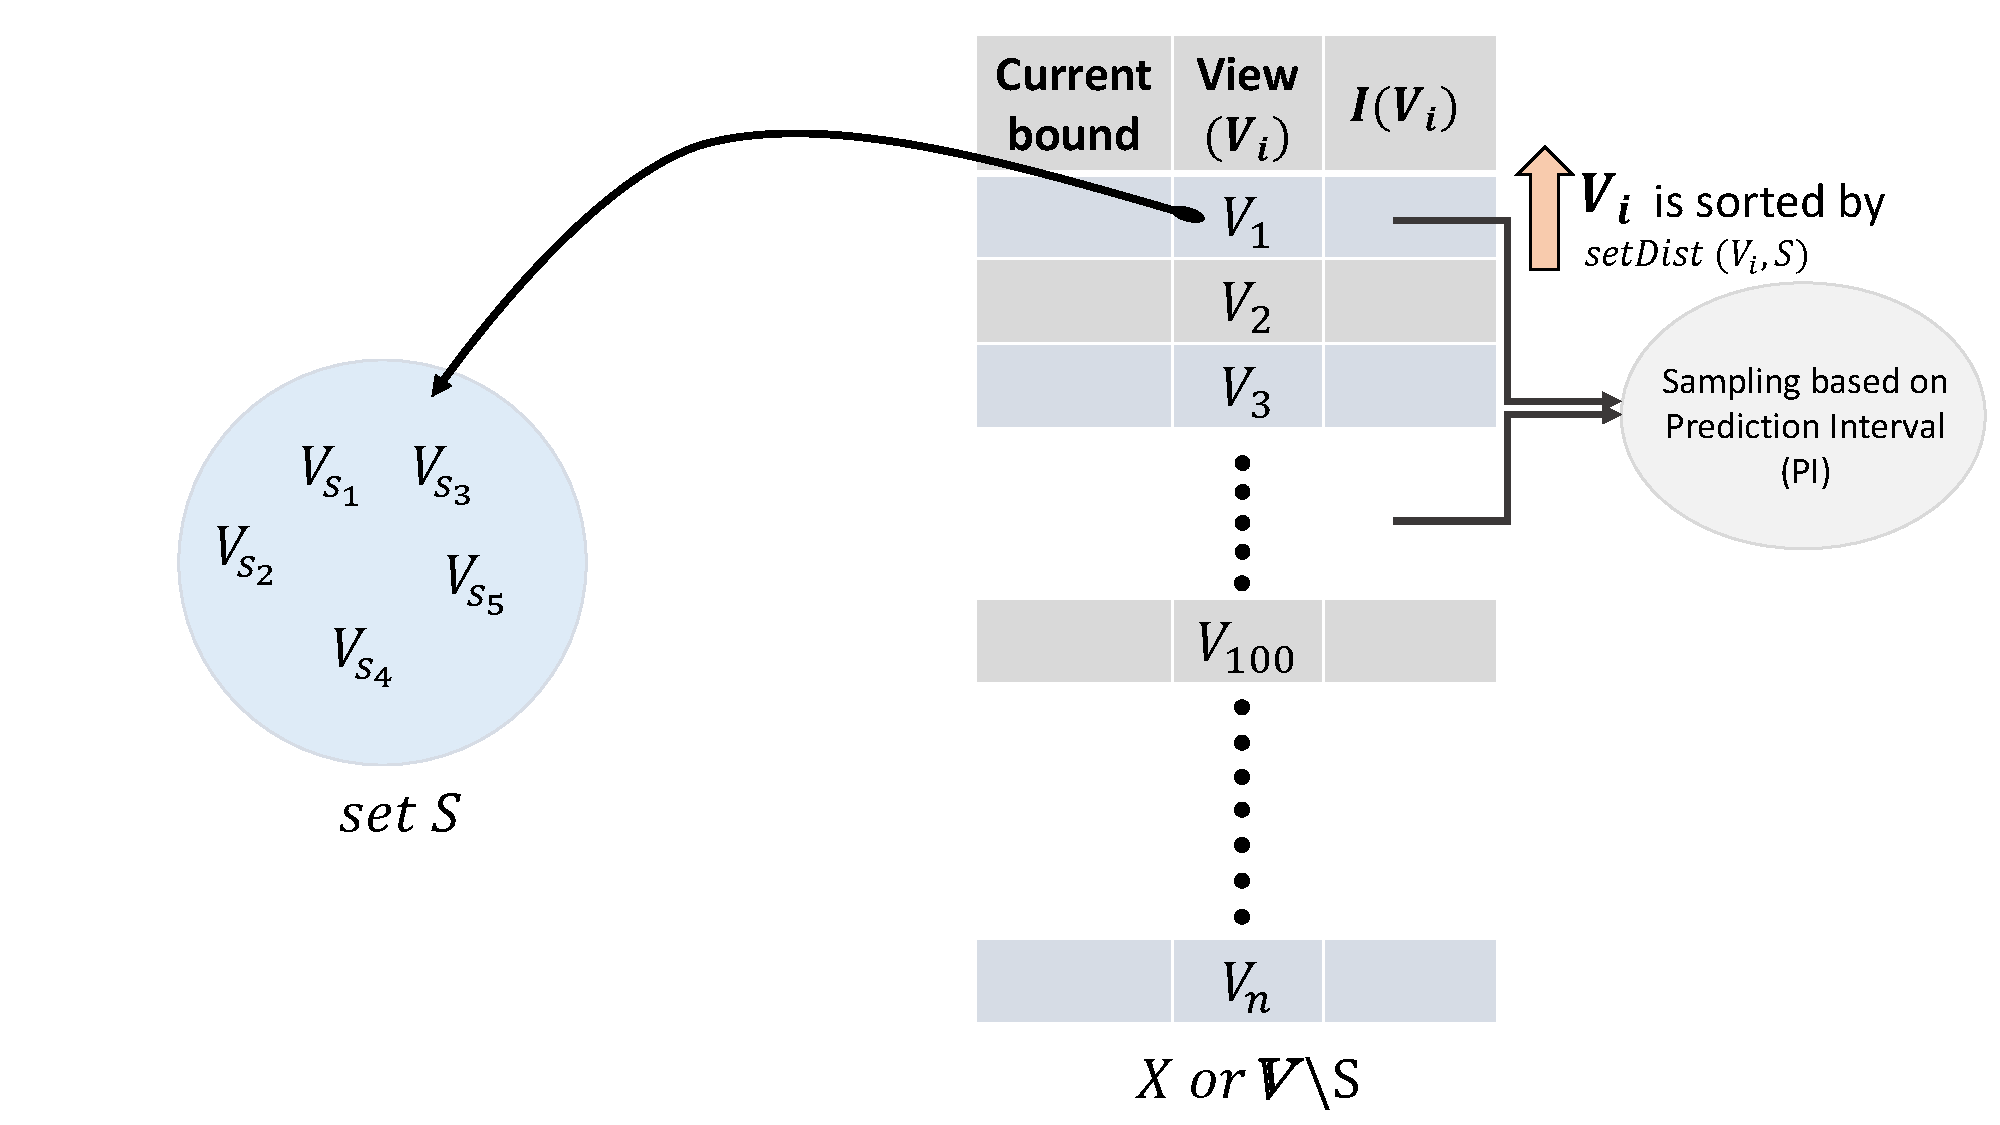
\includegraphics[width=3in]{figures/results/dSwap-Pruning}
%	\caption{dSwap-Pruning: Each candidate view has importance score and $ current bound $. The importance score of view will be generated only for view which its utility score is able to improve set $S$ while using $currentbound$ }
%	\label{fig:dSwap-Pruning}
%\end{figure}

%The idea behind pruning scheme is to minimize the query execution, which is by early prune low quality views. There are two main parameters in pruning scheme: 1) weight of $\lambda$ and 2) the max bound value $I_u$. 

%The weight of $\lambda$ is important due to it determines the contribution of importance score and diversity score. For instance, assume that an analyst wants to get set of views from view recommendation and she uses $\lambda$ = 0.7. The $\lambda$ value equal to 0.7 means that the diversity contribution to the utility score is 70\% and the contribution of importance score will be 30 \%, as it can be seen in equation \ref{objectif_function}. Thus, by setting the $\lambda$ to higher value, the contribution of importance score will be lower and more queries are pruned. This $\lambda$ value is determined by analyst, however, in this experiement 0.5 is used as the default. 